\documentclass[../main]{subfiles}

\begin{document}

To achieve this specific task utilizing GANs, a few considerations regarding the model's architecture need to be made.  REPHRASE: Primarily, the architecture must eliminate the problem of using a model made for continuous spaces on the textual domain, as is the case when generating movie reviews.  In addition, the model must be able to generate reviews under the intended sentiment, i.e. whether the review should be positive or negative.  To overcome the first concern, we decided to focus on the usage of word embeddings, rather than reinforcement learning. Regarding the sentiment parameter, there was the option to implement GAN2Vec's conditional variation or to modify a different architecture to comply with the idea of Conditional GANs. We settled on the latter, as it allowed us to partially implement an established architecture, while also being able to extend the existing approach to fit the task at hand.

\subsection{LaTextGAN \cite{latextgan}}
The LaTextGAN architecture was proposed in 2019 to adapt GANs to discrete spaces without the need to use Reinforcement Learning Techniques. Unlike vanilla GANs, LaTextGAN consists of a GAN component and an additional Variational Autoencoder, which in itself is further comprised of two sub-components: an Encoder and a Decoder.  

The Generator and Discriminator components in LATextGAN are realized using LSTM cells in a ResNet architecture.  It is important to note that the GAN component uses Earth Mover Distance and thus falls in the class of Wasserstein GANs. The Variational Autoencoder also utilizes LSTM cells to process the input sample at each time step and to model the long-term dependencies between words.  At the embedding layer (colored orange in Figure 2) of the VAE, the sample is encoded as a low-dimensional \textit{real} vector in the latent space. This representation is the key to circumventing the problem of using GANs on discrete domains and enables backpropagation.


\begin{figure}[h]
	\centering
	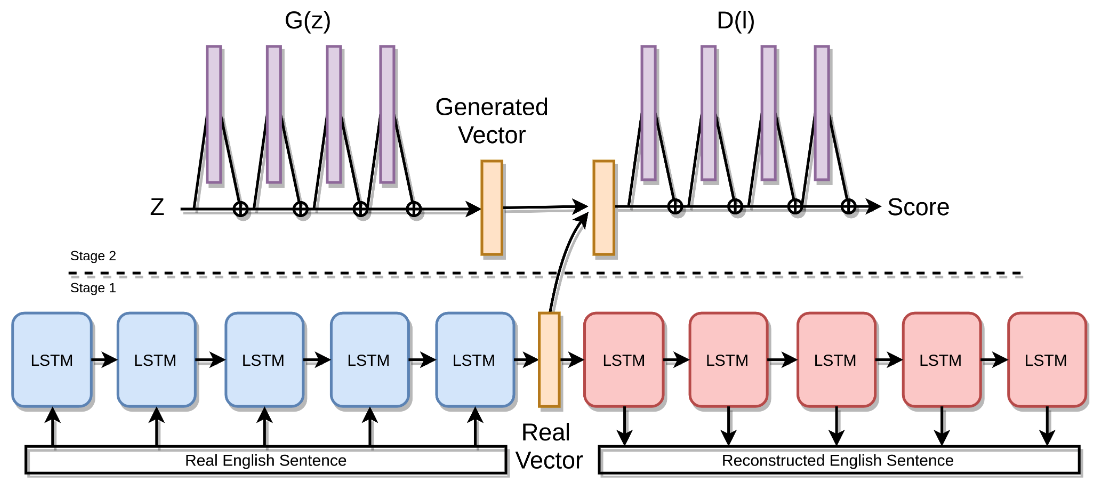
\includegraphics[scale=0.3]{LaTextGAN}
	\caption{The basic LaTextGAN architecture}
\end{figure}

Due to the additional VAE component, training has to occur in two distinct stages. Stage 1 focuses solely on the VAE, while the GAN is fixed. During Stage 2, the trained encoder and decoder are used to transform the discrete textual representation into real vectors and vice versa. The Generator no longer is tasked with generating novel sentences, but rather real-valued latent representations. To accommodate this modality change, the Discriminator is trained on the latent encoding of the training samples, to score the plausibility of the generated encoding to be a real sentence. The decoder can later be used to transform the latent vector back into natural language.

\subsection{Final Architecture}
Underlying our generative model is the LaTextGAN architecture, however, adapted to fit the specific task definition, i.e. generating plausible, opinionated movie reviews, conditioned on the given sentiment parameter (positive/negative).

\subsubsection{Variational Autoencoder}

\subsubsection{Generative Adversarial Network}

\end{document}